\documentclass{scrartcl}
\usepackage[mathletters]{ucs}
\usepackage[utf8x]{inputenc}
\usepackage{amssymb}
\usepackage{amsmath}
\usepackage[usenames]{color}
\usepackage{hyperref}
\usepackage{wasysym}
\usepackage{graphicx}
\usepackage[normalem]{ulem}
\usepackage{enumerate}

\usepackage{listings}

\lstset{ %
basicstyle=\footnotesize,       % the size of the fonts that are used for the code
showspaces=false,               % show spaces adding particular underscores
showstringspaces=false,         % underline spaces within strings
showtabs=false,                 % show tabs within strings adding particular underscores
frame=single,                   % adds a frame around the code
tabsize=2,                      % sets default tabsize to 2 spaces
breaklines=true,                % sets automatic line breaking
breakatwhitespace=false,        % sets if automatic breaks should only happen at whitespace
}


\title{initial dataset}
\date{dinsdag 08 december 2020}
\author{}

\begin{document}

\maketitle

		\section{initial dataset}

Created vrijdag 13 november 2020



\subsection{Form}

The dataset given where taken with a microscopic camera at Sirris. These images were in good lighting conditions for the measurement, but had a lot of extra "unwanted" features on it. The background was very like the wear and the rest of the tool insert. 

Every insert that was measured had a little mark on one side to mark the a and b. Sadly the information about what the marker meant is lost. To find the corresponding values, the inserts where once again put through a microscopic camera and the new pictures where compared against the old ones. 



While again checking the inserts out, a new dataset is created since this didn't ask much more time. During this proces there is also a new way of separating the sides of the inserts. There is a bullet at one side on every insert. This is an easy way to recognise a side and wont dissapear like the marker line. 







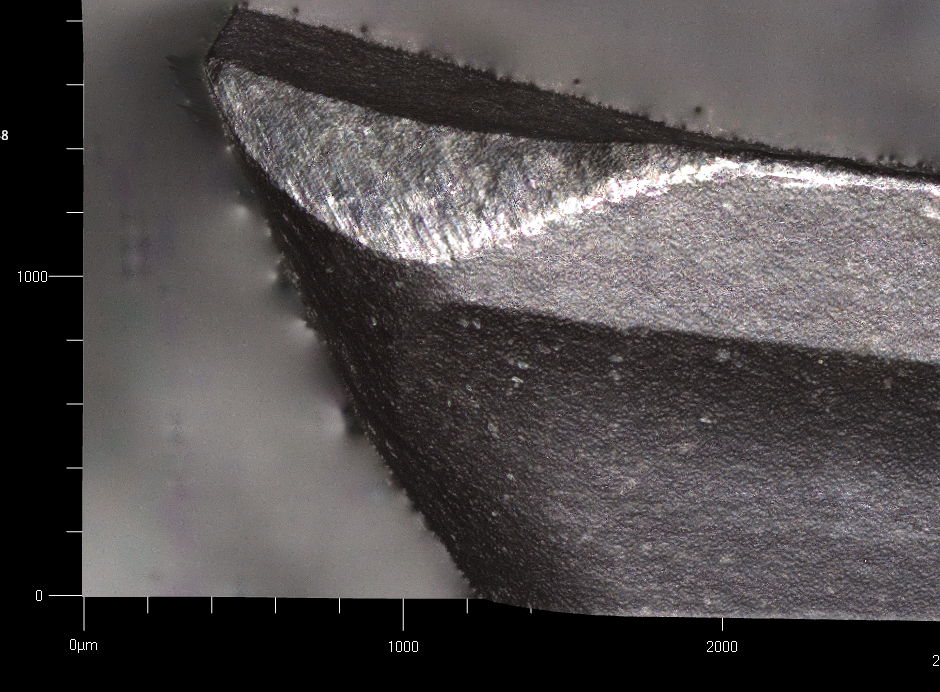
\includegraphics[width=3.125000in, keepaspectratio=true]{./initial_dataset/initial dataset pictuer.PNG}





\end{document}
